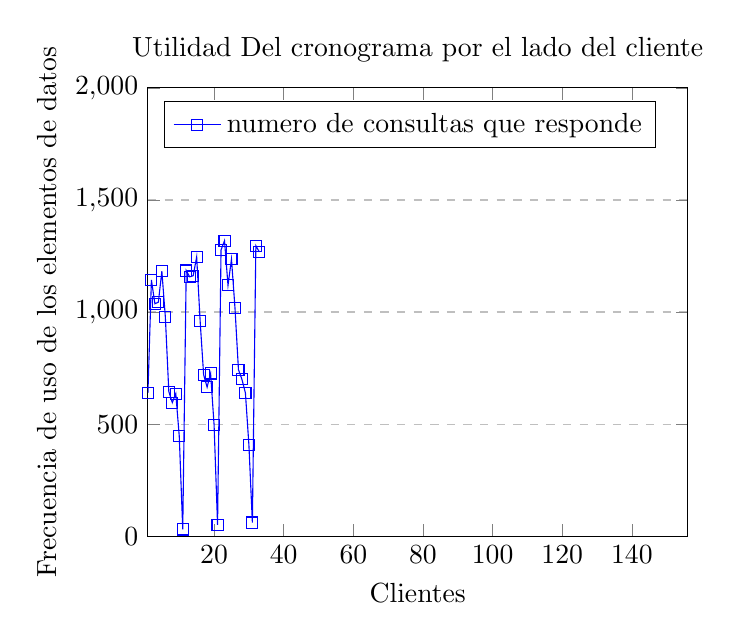
\begin{tikzpicture}
\begin{axis}[
    title={Utilidad Del cronograma por el lado del cliente},
    xlabel={Clientes},
    ylabel={Frecuencia de uso de los elementos de datos},
    xmin=1, xmax=156,
    ymin=0, ymax=2000,
    xtick={},
    ytick={},
    legend pos=north west,
    ymajorgrids=true,
    grid style=dashed,
]

\addplot[
    color=blue,
    mark=square,
    ]
    coordinates {
    %USO EXACTO
    (1,639)
(2,1143)
(3,1037)
(4,1044)
(5,1182)
(6,979)
(7,645)
(8,596)
(9,636)
(10,446)
(11,30)
(12,1185)
(13,1157)
(14,1162)
(15,1246)
(16,959)
(17,720)
(18,665)
(19,726)
(20,497)
(21,51)
(22,1277)
(23,1318)
(24,1119)
(25,1236)
(26,1019)
(27,743)
(28,700)
(29,639)
(30,408)
(31,61)
(32,1296)
(33,1268)
    };
    \legend{numero de consultas que responde}

\end{axis}
\end{tikzpicture}

